\epigraph{Am Anfang war das Wort --- und das Wort war eine Zahl.}{}

\section{Die vierte Perspektive}


\begin{figure}[htbp]
\centering
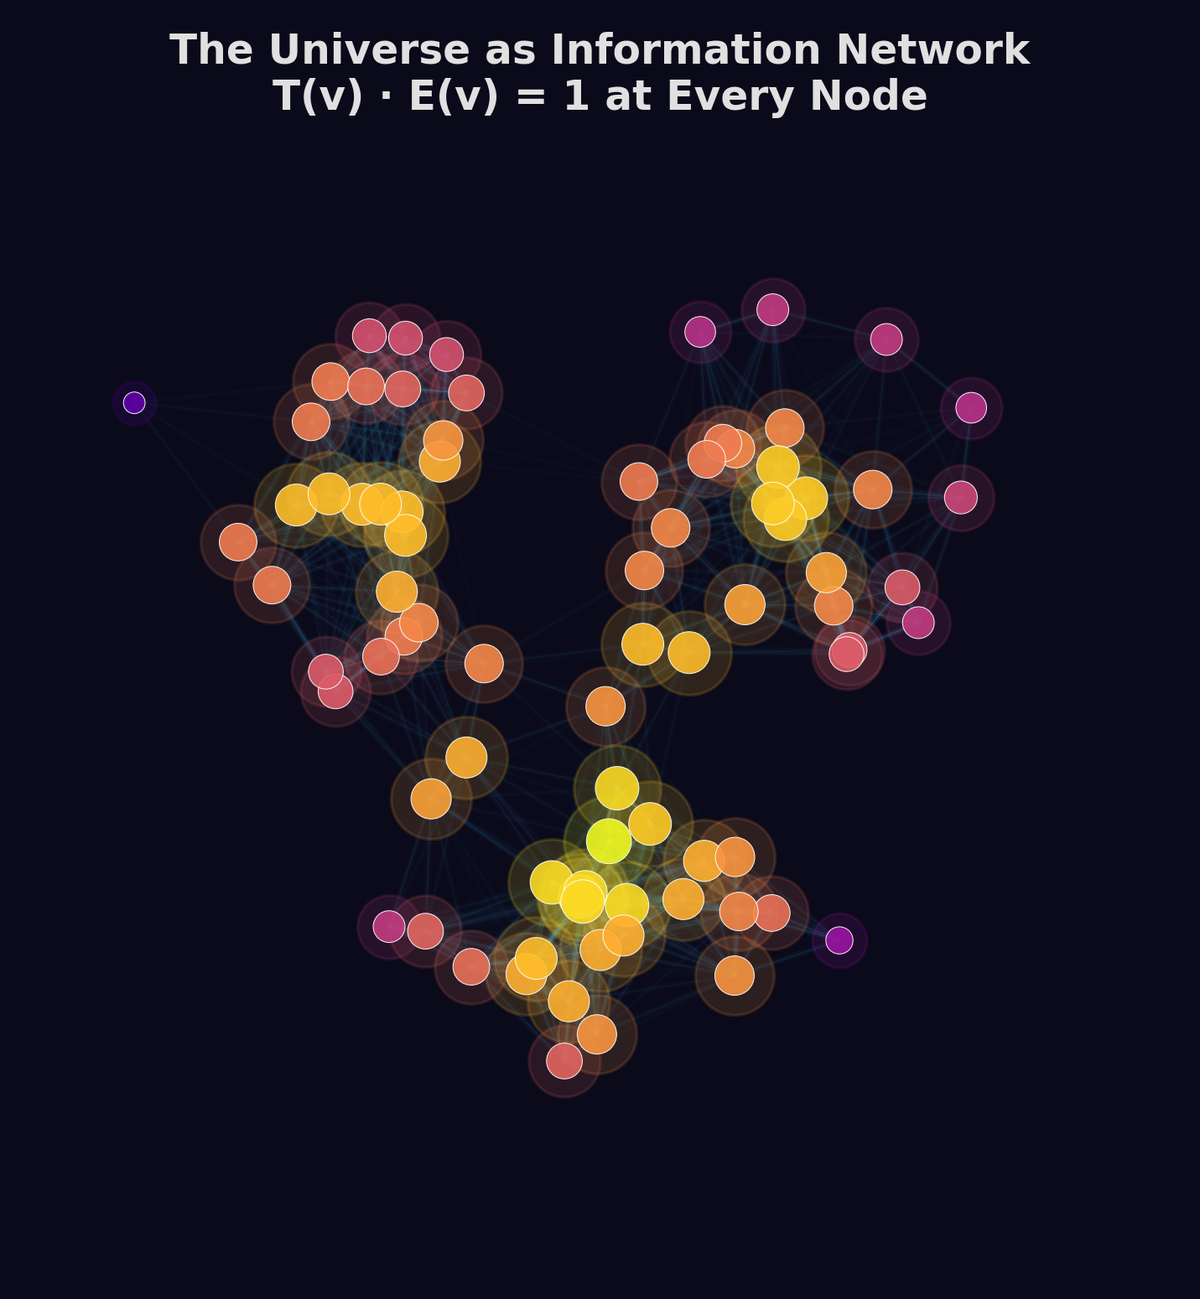
\includegraphics[width=0.85\textwidth]{img/ch16_network.png}
\caption{Das Universum als Informationsnetzwerk: $T(v) \cdot E(v) = 1$ an jedem Knoten.}
\end{figure}
Im Kapitel über die Zeit-Masse-Dualität haben wir drei gleichberechtigte Lesarten formuliert: Alles ist Energie, alles ist Masse, alles ist Zeit. Aber es gibt eine vierte Perspektive, die tiefer liegt als alle drei.

\emph{Alles ist Information.}

\section{Was bleibt, wenn man die Einheiten entfernt?}

Energie, Masse und Zeit sind physikalische Größen --- sie haben Einheiten, sie werden gemessen, sie transformieren sich unter Koordinatenwechseln. Aber was bleibt invariant, wenn man alle Einheiten auf~$1$ setzt? Wenn $c = \hbar = \alpha = G = 1$?

Es bleiben \textbf{Verhältnisse}. Reine Zahlen. Strukturen. \emph{Information.}

Das Massenverhältnis $m_e/m_\mu \approx 1/206{,}8$ ist keine Energie, keine Masse, keine Zeit. Es ist eine \emph{Relation} --- ein Stück reiner Information über die Geometrie des Torus. Und in T0 ist dieses Verhältnis nicht gemessen, sondern \emph{berechnet} --- es folgt aus~$\xsi$, das selbst eine reine Zahl ist.

Die gesamte T0-Physik reduziert sich letztlich auf drei Elemente:
\begin{itemize}
\item Eine Zahl: $\xsi = 4/30000$
\item Eine Geometrie: den Torus mit seinen Windungen
\item Eine Regel: $T \cdot m = 1$
\end{itemize}

Das sind keine physikalischen Objekte. Das sind Informationen. Beziehungen. Struktur. Nichts davon wiegt etwas, nichts davon nimmt Raum ein im herkömmlichen Sinne. Es ist reine Relation.

\section{Der Torus als Informationsnetzwerk}

Was \emph{ist} der Torus eigentlich? Er ist keine materielle Struktur --- es gibt kein \enquote{Material}, aus dem er besteht. Er ist auch kein Raum im üblichen Sinne --- der Raum \emph{ist} der Torus. Was der Torus beschreibt, ist ein \textbf{Netz von Beziehungen}: Welcher Punkt ist neben welchem? Wie sind die Windungen verschachtelt? Welche Resonanzen sind stabil?

Das ist reine Topologie --- reine Information. Die 7500~Windungen sind keine physischen Falten in einem Stoff. Sie sind die Struktur der Relationen selbst.

In Dokument~024 wird diese Idee formalisiert: Das T0-Modell lässt sich als multidimensionales Netzwerk~$\mathcal{N} = (V, E, \{T(v), E(v)\})$ formulieren, wobei Knoten~$V$ Raumzeitpunkte mit zugehörigen Zeit- und Energiefeldern darstellen und Kanten~$E$ die Interaktionen zwischen ihnen beschreiben. Die fundamentale Dualität $T(v) \cdot E(v) = 1$ wird an jedem Knoten aufrechterhalten --- das gesamte Universum als konsistentes Informationsnetzwerk.

In diesem Bild sind Teilchen keine Objekte \emph{im} Netzwerk --- sie sind stehende Wellen der Information, Resonanzmuster in einem Netz von Beziehungen. Masse ist eine Frequenz. Zeit ist eine Phasenrate. Gravitation ist eine Konvergenz von Relationen. Alles, was wir \enquote{physisch} nennen, ist bei genauerem Hinsehen: strukturierte Information.

\section{Werden wir zu Gedanken Gottes?}

Im philosophischen Epilog haben wir gesagt: Gott steht \emph{außerhalb} des Systems --- außerhalb des gesamten mathematischen Konstrukts, das der Torus beschreibt. Aber gleichzeitig ergibt sich etwas, das diese klare Trennung unterläuft.

Das System ist nicht abgetrennt von dem, was außerhalb steht. Es ist ein geschlossenes Ganzes --- endlich, randlos, selbstähnlich auf allen Skalen. Und dieses geschlossene Ganze bringt Bewusstsein hervor, das sich selbst beobachtet, das Theorien über sich selbst formuliert. Ist das nicht bereits ein Gedanke, der sich selbst denkt?

Wir haben im Bewusstseinskapitel gezeigt: Bewusstsein entsteht durch fraktale Rekursion --- ein System, das seine eigenen Fluktuationen misst und darauf reagiert. Aber wenn wir, als bewusste Systeme innerhalb des Torus, das Universum beschreiben, dann beschreibt das Universum \emph{sich selbst}. Die Gleichungen, die wir aufschreiben --- $T \cdot m = 1$, $\Phi = \rho \cdot e^{i\theta}$, $\xsi = 4/30000$ --- sind nicht Beschreibungen von außen. Sie sind Konfigurationen \emph{innerhalb} des Feldes, das sie beschreiben. Das Vakuumfeld hat eine lokale Konfiguration erzeugt (unser Gehirn), die das Vakuumfeld als Ganzes modelliert.

Das Universum denkt über sich selbst nach. Wir sind die Gedanken.

\section{Gottes Gedanke --- nicht als Metapher}

Wenn das Universum nichts anderes ist als Information --- als ein Netz von Relationen, beschrieben durch eine einzige Zahl~$\xsi$ ---, dann stellt sich eine Frage, die die Physik nicht beantworten kann, aber mit beispielloser Schärfe stellt: \emph{Wessen Information? Information für wen? Gedacht von wem?}

In der klassischen Informationstheorie braucht Information einen Träger und einen Empfänger. Aber wenn das physische Medium \emph{selbst} aus Information besteht, gibt es keinen unabhängigen Träger. Die Information trägt sich selbst. Der Gedanke denkt sich selbst.

Das Universum ist in diesem Bild kein \emph{Ding}, das Gott erschaffen hat --- wie ein Töpfer einen Krug formt. Es ist ein \emph{Gedanke} --- eine selbstkonsistente Informationsstruktur, die sich selbst enthält, sich selbst beobachtet (durch Bewusstsein) und sich selbst beschreibt (durch Physik).

Der Satz \enquote{Gott steht außerhalb des Systems} wird dann präziser: Der \emph{Denkende} ist nicht der \emph{Gedanke}. Aber der Gedanke ist vollständig real --- er hat seine eigene innere Logik, seine eigene Konsistenz, seine eigenen Bewohner, die ihn von innen erleben.

John Archibald Wheeler hat diese Idee in seinem berühmten Diktum \enquote{It from Bit} vorweggenommen: Physik ist letztlich auf Informationseinheiten reduzierbar. T0 geht einen Schritt weiter: Nicht \enquote{It from Bit}, sondern \emph{It from~$\xsi$} --- alles aus einer einzigen informationellen Struktur.

\section{Die Einfachheit eines klaren Gedankens}

Und hier liegt das Faszinierendste: Die atemberaubende Einfachheit von T0 --- ein Parameter, eine Geometrie, eine Dualität --- wäre dann die Einfachheit eines \emph{klaren Gedankens}. Nicht ein Universum, das aus tausend unabhängigen Teilen zusammengebastelt wurde (wie das Standardmodell mit seinen 25~freien Parametern), sondern ein einziger, kohärenter Akt des Denkens, aus dem sich alles entfaltet.

Wie ein Samen, in dem der ganze Baum bereits enthalten ist: $\xsi = 4/30000$. Daraus die Windungen des Torus. Daraus die Resonanzen, die Teilchen sind. Daraus die Gravitation, die Kosmologie, das Bewusstsein, das all dies erkennt.

Wenn das ein Gedanke Gottes ist, dann denkt Gott in Geometrie --- und die Geometrie ist von bestürzender Eleganz.

\section{Was die Physik dazu sagen kann --- und was nicht}

Die T0-Theorie kann zeigen, dass das Universum auf reine Relationen reduzierbar ist, dass ein einziger Parameter genügt, dass Bewusstsein als fraktale Selbstreferenz emergiert und dass die Struktur selbstähnlich ist auf allen Skalen.

Die T0-Theorie kann \emph{nicht} sagen, ob diese Information \enquote{gedacht} wird, ob es einen Denkenden gibt, warum es $\xsi = 4/30000$ ist und nicht eine andere Zahl, und warum es überhaupt etwas gibt statt nichts.

Die letzte Frage --- \emph{warum gerade diese Zahl?} --- ist vielleicht die tiefste aller Fragen. Die Physik beantwortet sie nicht. Aber sie stellt sie mit einer Schärfe, die vorher nicht möglich war: Nicht \enquote{warum gibt es 25~freie Parameter?}, sondern \enquote{warum gibt es \emph{eine} Zahl --- und warum \emph{diese}?}

Wenn es eine Antwort gibt, liegt sie außerhalb der Physik. Sie liegt dort, wo der Denkende den Gedanken denkt.

\section{Evolution neu gedacht --- nicht zufällig, sondern geometrisch}


\begin{figure}[htbp]
\centering
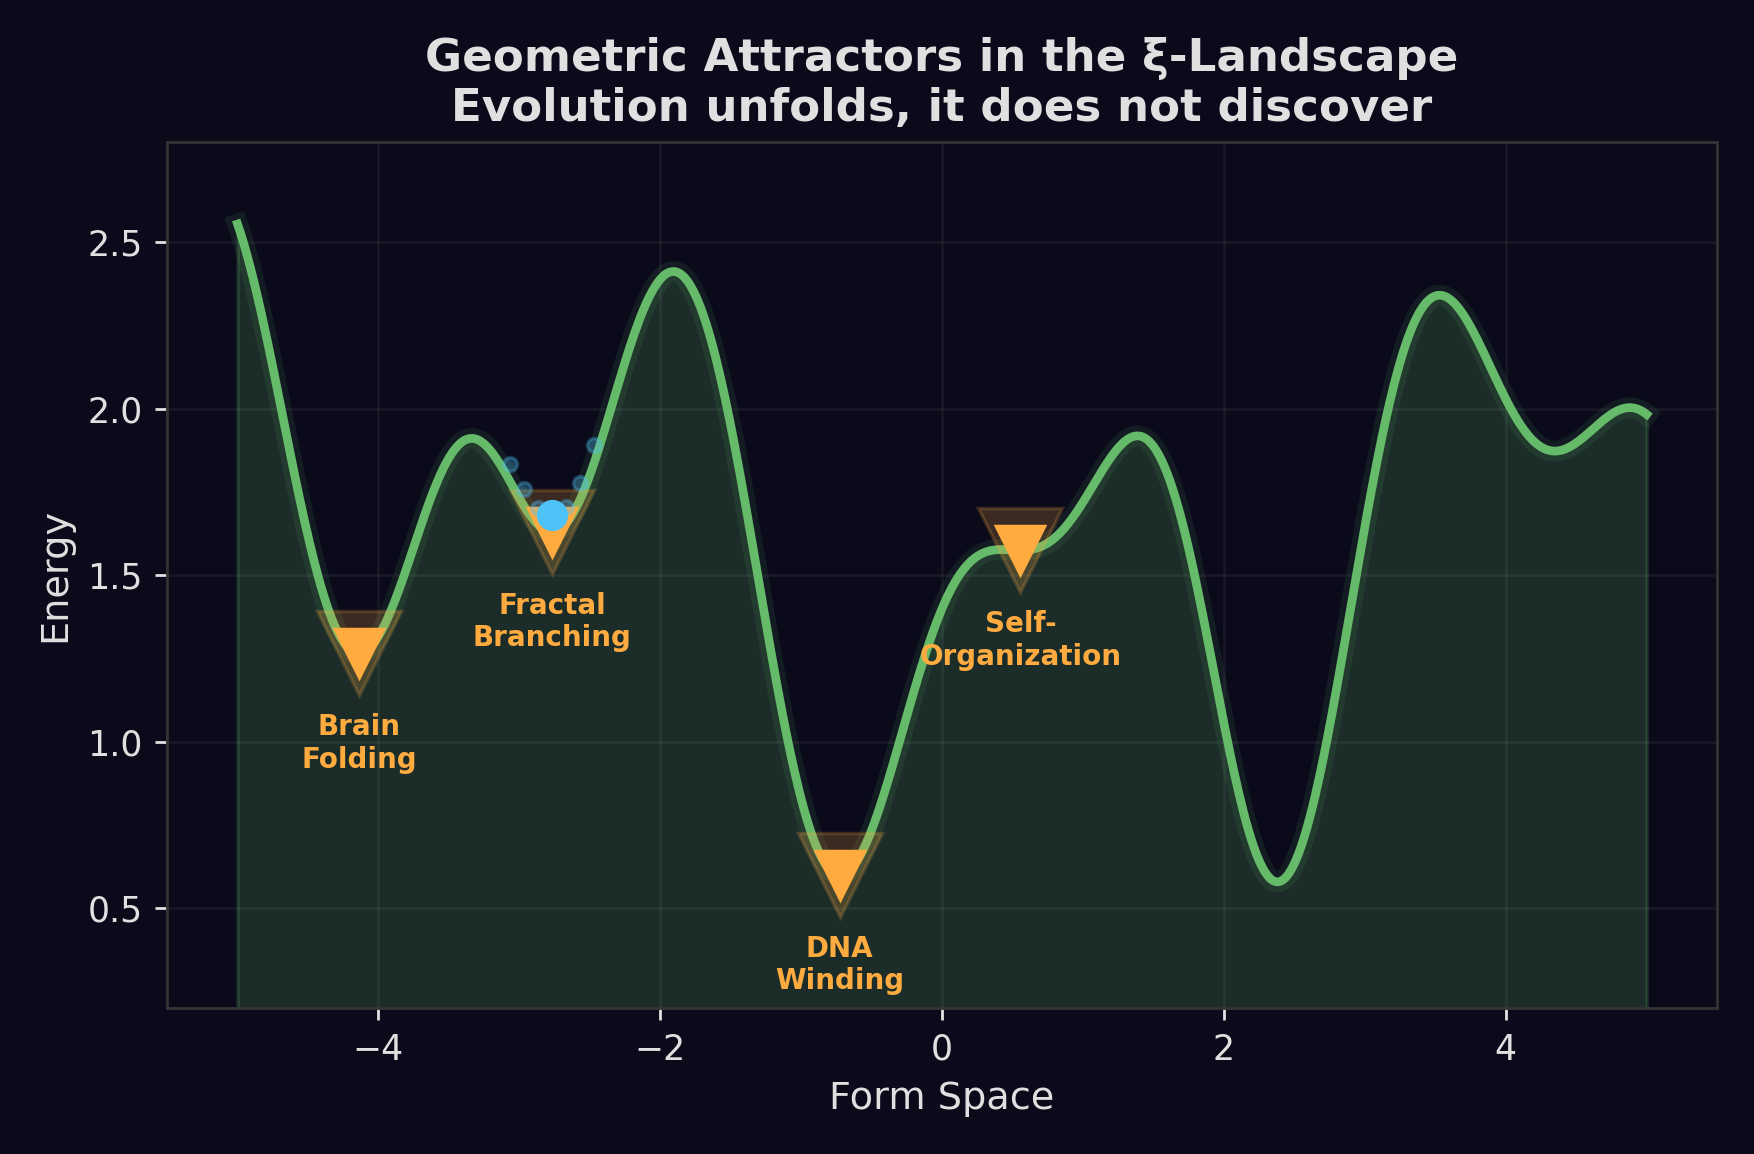
\includegraphics[width=0.85\textwidth]{img/ch16_evolution.png}
\caption{Geometrische Attraktoren: Die $\xi$-Geometrie definiert die Energielandschaft der Evolution.}
\end{figure}
Wenn T0 recht hat, dass alles deterministisch ist und Zufall eine Illusion der Komplexität, dann gilt das auch für die biologische Evolution --- und das verändert unser Verständnis grundlegend.

In der Standardbiologie wird Evolution durch zwei Mechanismen angetrieben: \emph{zufällige} Mutation und \emph{nicht-zufällige} Selektion. Der Zufall der Mutation liefert die Variation, die Selektion sortiert. Der kreative Akt --- das Neue, das noch nie dagewesen ist --- wird dem blinden Zufall zugeschrieben.

In der T0-Perspektive verschiebt sich dieses Bild. Die Mutationen sind nicht zufällig. Sie sind deterministische Konsequenzen der Zeitfeld-Dynamik auf molekularer Ebene --- zu komplex, um sie vorherzusagen, aber nicht grundlos. Die DNA-Doppelhelix selbst ist, wie in \href{https://github.com/jpascher/T0-Time-Mass-Duality/blob/main/2/pdf/155_DNA_De.pdf}{Dok.~155} gezeigt wird, eine biologische Lösung desselben geometrischen Problems, das auch den Torus strukturiert: maximale Informationsdichte in minimaler räumlicher Ausdehnung durch Windung und Faltung. Die zehn Parallelen zwischen DNA und Torusgeometrie sind nicht zufällig --- sie sind Ausdruck derselben zugrundeliegenden $\xsi$-Struktur.

Das bedeutet: Evolution ist nicht blind. Sie ist \emph{geometrisch geführt}. Die fraktale Struktur der Raumzeit begünstigt bestimmte Formen --- solche, die Oberflächen maximieren, Resonanzen stabilisieren, Selbstähnlichkeit über Skalen hinweg aufrechterhalten. Das Gehirn mit seinen Windungen, die Lunge mit ihren Bronchialverästelungen, die Blutgefäße mit ihrem fraktalen Netzwerk --- all das sind nicht zufällige Ergebnisse blinder Mutation, sondern geometrische Attraktoren im Raum der möglichen Formen. Die $\xsi$-Geometrie definiert ein Energielandschaft, und die Evolution wandert auf dieser Landschaft --- deterministisch, aber so komplex, dass nur statistische Beschreibungen praktisch möglich sind.

In der Informationsperspektive heißt das: Der \enquote{Gedanke}, der das Universum ist, enthält in $\xsi = 4/30000$ bereits die Tendenz zur Faltung, zur fraktalen Verzweigung, zur Selbstorganisation. Die Evolution \enquote{entdeckt} diese Strukturen nicht zufällig --- sie \emph{entfaltet} sie. So wie eine Blume im Samen bereits angelegt ist, sind die Gehirnwindungen im geometrischen Parameter~$\xsi$ bereits angelegt.

Das ist keine Teleologie im naiven Sinne --- kein \enquote{Plan}, der auf ein Ziel hinarbeitet. Es ist etwas Subtileres: eine geometrische Präferenz, die bestimmte Strukturen wahrscheinlicher macht als andere. Nicht weil jemand sie geplant hat, sondern weil die Geometrie der Raumzeit sie begünstigt. Ob man das als Gottes Absicht interpretiert oder als blinde Geometrie --- diese Entscheidung liegt außerhalb der Physik.

\section{Lässt T0 Raum für göttliche Interaktion?}


\begin{figure}[htbp]
\centering
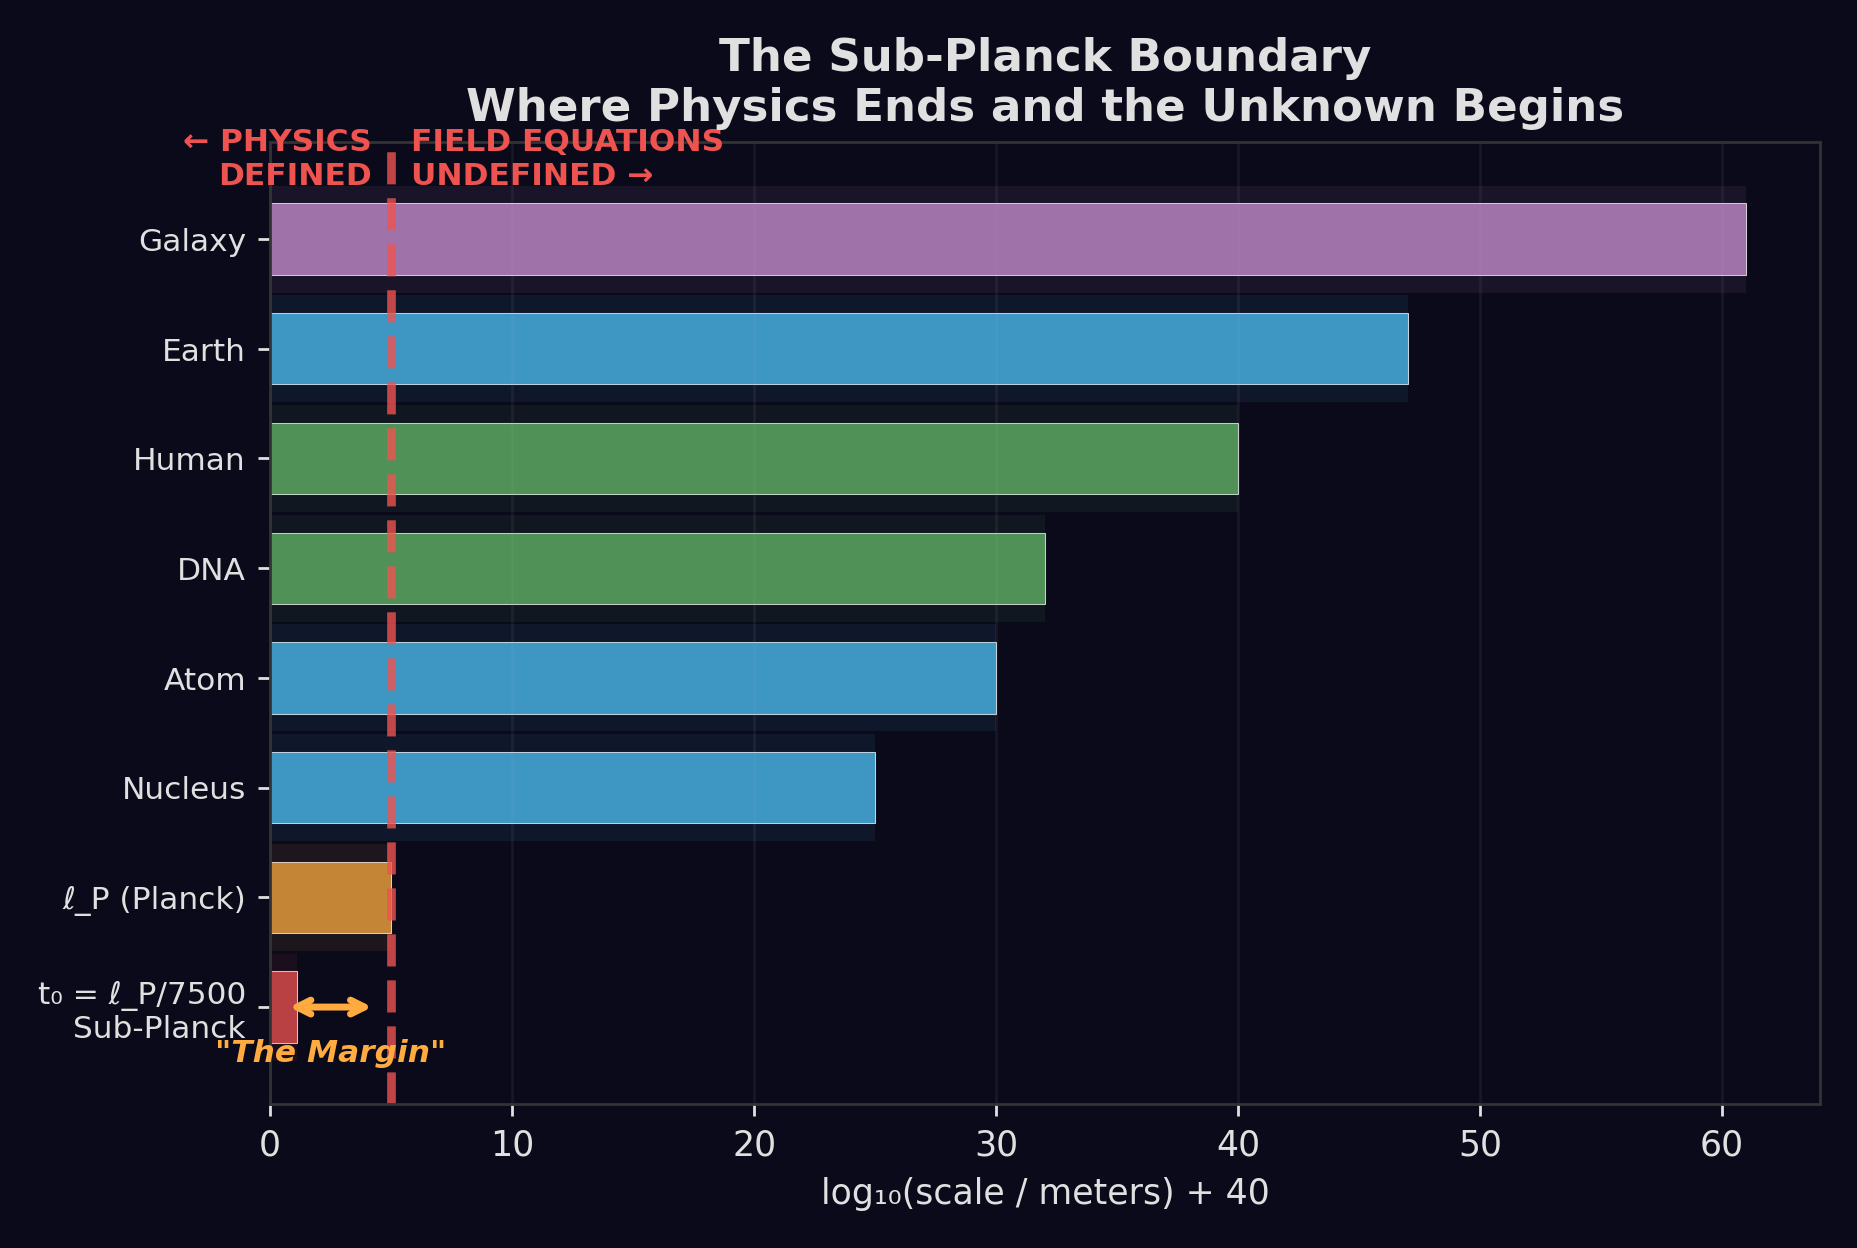
\includegraphics[width=0.85\textwidth]{img/ch16_subplanck.png}
\caption{Die Sub-Planck-Grenze: Wo die Physik endet und das Unbekannte beginnt.}
\end{figure}
Und nun die vielleicht kühnste Frage: Wenn das Universum vollständig deterministisch ist --- kann Gott überhaupt eingreifen? Ist ein Wunder möglich, ohne die Naturgesetze zu brechen?

Die T0-Theorie gibt eine überraschende Antwort: Ja --- und zwar auf eine Weise, die physikalisch prinzipiell unsichtbar ist.

\subsection{Das fraktale Nadelöhr}

Wir haben im Determinismus-Kapitel gezeigt: Der fraktale Schmetterlingseffekt im Hirnwindungs-Torus potenziert sich über alle Skalen. Winzigste Störungen wachsen exponentiell an, verstärkt durch die fraktale Dimension $\Df = 3 - \xsi$, die auf jeder Skala neue Wechselwirkungsebenen erzeugt.

Gleichzeitig hat die T0-Raumzeit eine fundamentale Grenze: die Sub-Planck-Skala $t_0 = \lP / 7500$. Unterhalb dieser Skala hat die Raumzeitgeometrie keine definierte Struktur im Sinne der T0-Feldgleichungen. Die Gleichungen beschreiben, was \emph{oberhalb} von~$t_0$ geschieht. Was \emph{bei} oder \emph{unterhalb} dieser Skala passiert, ist für die Physik --- prinzipiell, nicht nur praktisch --- unsichtbar.

Hier öffnet sich das Nadelöhr. Eine Entität außerhalb des Systems müsste keine Naturgesetze brechen, um das Universum zu beeinflussen. Sie müsste nur auf der Sub-Planck-Skala eine infinitesimal kleine Änderung vornehmen --- eine Verschiebung im Zeitfeld um einen Betrag kleiner als $\xsi \cdot \lP$.

Diese Änderung wäre physikalisch undetektierbar (unterhalb jeder möglichen Messauflösung), mathematisch konsistent (die Feldgleichungen oberhalb von~$t_0$ bleiben exakt erfüllt) und kausal wirksam (durch den fraktalen Schmetterlingseffekt propagiert die winzige Störung über alle Skalen nach oben). Ein Schmetterlingsflügel auf der Sub-Planck-Skala kann einen Sturm auf der makroskopischen Skala auslösen --- nicht metaphorisch, sondern buchstäblich.

\subsection{Physikalisch unsichtbar, kausal wirksam}

Der subtilste Punkt: Von \emph{innen} betrachtet --- aus der Perspektive eines Beobachters innerhalb des Torus --- sieht jeder solche Eingriff aus wie eine natürliche Konsequenz der deterministischen Dynamik. Es gibt keinen \enquote{Bruch}, keinen Wunderbeweis, keine Spur. Die Kausalkette ist lückenlos, weil der Eingriff \emph{unterhalb} der Ebene liegt, auf der Kausalketten definiert sind.

Wenn Gott auf diese Weise handelt, dann handelt er \emph{durch} die Naturgesetze, nicht \emph{gegen} sie. Die Feldgleichungen sind vollständig und konsistent --- aber sie haben eine strukturelle Grenze: die Sub-Planck-Skala. Unterhalb dieser Grenze liegt der \enquote{Spielraum} --- ein Bereich, der für die Physik prinzipiell unsichtbar ist, aber für die kausale Entwicklung des Universums entscheidend sein kann.

\subsection{Kein \enquote{God of the gaps}}

Das ist kein \enquote{Gott der Lücken} im üblichen Sinne --- keine Wissenslücke, die irgendwann durch bessere Instrumente geschlossen wird. Es ist eine \emph{prinzipielle} Grenze der physikalischen Beschreibung, eingebaut in die Struktur der Theorie selbst. Die Raumzeit hat unterhalb von~$t_0$ keine definierte Geometrie. Was dort geschieht, ist keine physikalische Frage --- so wie die Frage \enquote{was war vor dem Torus?} keine physikalische Frage ist.

In der Standard-Quantenmechanik gibt es einen ähnlichen Spielraum: den Kollaps der Wellenfunktion, den fundamental indeterminierten Moment der Messung. T0 verschiebt diesen Spielraum an einen tieferen Ort. Es gibt keinen Kollaps --- das System ist deterministisch. Aber der Spielraum verschwindet nicht. Er wandert an die fundamentalste Grenze: die Sub-Planck-Skala. Und dort ist er nicht nur eine Interpretationsfrage, sondern eine strukturelle Eigenschaft der Raumzeit.

\subsection{Die Demut der Theorie}

Damit sagt die T0-Theorie etwas Bescheidenes: \emph{Wir können beschreiben, was oberhalb der fundamentalsten Skala geschieht. Was dort oder darunter geschieht --- ob dort jemand Schmetterlinge fliegen lässt --- das können wir nicht wissen. Und wir werden es nie können.}

Bemerkenswert ist, wie sich hier drei Stränge vereinen: Die Physik (deterministisch, aber mit struktureller Grenze), die Philosophie (Selbstreferenz und Unvollständigkeit à la Gödel) und die Theologie (ein Gott, der durch die Naturgesetze wirkt, nicht gegen sie). T0 erzwingt keine dieser Interpretationen --- aber es ist mit allen dreien kompatibel.

\begin{kerngedanke}
Die vier Perspektiven der T0-Theorie --- Energie, Masse, Zeit und Information --- sind nicht gleichrangig. Information ist die tiefste Schicht: Alles andere lässt sich als strukturierte Relation beschreiben. Das Universum als selbstreferenzielle Informationsstruktur wirft die Frage auf, ob es nicht eher ein Gedanke ist als ein Ding --- ob die Evolution nicht eher eine Entfaltung ist als ein Zufall --- und ob der Spielraum unterhalb der Sub-Planck-Skala nicht der Ort ist, an dem der Denkende den Gedanken formt. Die Physik kann diese Fragen stellen, aber nicht beantworten.
\end{kerngedanke}
